
%(BEGIN_QUESTION)
% Copyright 2009, Tony R. Kuphaldt, released under the Creative Commons Attribution License (v 1.0)
% This means you may do almost anything with this work of mine, so long as you give me proper credit

Write a simple relay ladder-logic (RLL) program in your PLC, where a discrete input bit (associated with an actual switch connected to an input channel) drives an internal coil (one that is not associated with a real-world discrete output channel):

$$\includegraphics[width=15.5cm]{i03693x01.eps}$$

Configure your HMI panel to display the status of this internal bit, through a ``lamp'' object on the HMI display.  This way, the HMI's ``lamp'' should ``energize'' when the real-world switch connected to the PLC is activated.

\vskip 20pt \vbox{\hrule \hbox{\strut \vrule{} {\bf Suggestions for Socratic discussion} \vrule} \hrule}

\begin{itemize}
\item{} Does your PLC have any special designations for bits not directly ``connected'' to real-world I/O points?
\end{itemize}



\vfil 

\noindent
PLC comparison:

\begin{itemize}
\item{} \underbar{Allen-Bradley Logix 5000}: all bits are named with tags, with the {\it tags window} being the place in the programming software where associations between tag names and I/O points may be viewed (if they exist at all).
\vskip 5pt
\item{} \underbar{Allen-Bradley SLC 500}: typically the {\it binary} file elements are used for internal bits (referenced with the letter {\tt B} as opposed to {\tt I} for inputs and {\tt O} for outputs).
\vskip 5pt
\item{} \underbar{Siemens S7-200}: typically the {\it bit memory} area is used for internal bits (referenced with the letter {\tt M} as opposed to {\tt I} for inputs and {\tt Q} for outputs).
\vskip 5pt
\item{} \underbar{Koyo (Automation Direct) DirectLogic}: typically the {\it control relay} memory area is used for internal bits (referenced with the letter {\tt C} as opposed to {\tt X} for inputs and {\tt Y} for outputs).
\end{itemize}

\underbar{file i03693}
\eject
%(END_QUESTION)





%(BEGIN_ANSWER)


%(END_ANSWER)





%(BEGIN_NOTES)


%INDEX% PLC, exploratory question (HMI programming)

%(END_NOTES)


